\section{Introduction}

The methodology proposed by \citet{Souza-Junior2023b} aims to achieve the semi-automatic estimation of dipole moments for individual grains, this is approached through a three-part methodology:

\begin{enumerate}
    \item \textbf{Data preprocessing:} Apply classic potential field data processing techniques, including the total gradient amplitude map (TGA). Employ image processing methods, such as histogram stretching, and an edge detection algorithm to identify and spatially isolate the magnetic field of each source into window data.

    \item \textbf{3D position estimation:} Estimate the 3D position of magnetic particles by applying the Euler deconvolution method to the data segment identified in the first step.

    \item \textbf{Magnetic moment inversion:} Execute the magnetic moment inversion in the data segment to determine the 3-component dipole moment vector. Which assumes a dipole model located in the position estimated with the Euler equation. 
\end{enumerate}

Performing the inversion separately for each data segment enhances computational efficiency, ensuring a quick solution to the linear inverse problem. However, it is important to acknowledge that stronger magnetic sources may influence the estimated positions and magnetic moment of nearby weaker ones. This understanding is crucial for refining the estimation process and ensuring robust results in magnetic parameter estimation.

%%%%%%%%%%%%%%%%%%%%%%%%%%%%%%%%%%%%%%%%%%%%%%%%%%%%%%%%%%%%%%%%%%%%%%%%%%%%%%%
\section{Methodology}

% The methodology proposed by \citet{Souza-Junior2023b} aimed to achieve the semi-automatic estimation of dipole moments for individual grains per image. This is approached through a three-part methodology. The initial step involves the application of classic potential field data processing, such as total gradient amplitude, coupled with image processing techniques like histogram stretching, equalization, and an edge detection algorithm. This enables the identification and spatial isolation of the magnetic field caused by each source. 

% Following that, attention shifts to the estimation of the 3D position of magnetic particles based on magnetic field measurements. This is carried out by applying the Euler deconvolution method to the data segment identified in the first step. In the final phase, the magnetic moment inversion process is executed. This entails estimating the 3-component dipole moment vector by inverting the magnetic field data assuming a dipolar model. The inversion is conducted separately for each data segment identified initially, which in theory ensures stability and computational efficiency in solving the linear inverse problem in a few seconds. 

% However, estimating the source's position based on Euler deconvolution revealed that stronger magnetic sources may influence the estimated positions of nearby weaker ones. Therefore, it becomes imperative to consider the interplay among the sources to estimate their magnetic parameters and position accurately. Understanding how these magnetic sources interact with each other is crucial for refining our estimation process and ensuring robust results in magnetic parameter estimation.

This study explores a new methodology to effectively manage interfering sources during the inversion process. Which is designed to mitigate the magnetic sources' interference and enhance the precision of the inversion analyses proposed by \citet{Souza-Junior2023b}.

\subsection{Magnetic inversion: interfering sources}

% \subsubsection{Iterative Euler deconvolution}

The proposed methodology aims to enhance the accuracy of window-based inversion analyses in magnetic data, particularly in scenarios where stronger magnetic sources could introduce distortions in the results. As mentioned earlier, the edge detection algorithm is applied to the TGA map to segment the data windows of the magnetic sources, which follow the descending order of blob magnitude. The latter is directly proportional to the magnetic signal of the sources, hence it might be used in the process to account for the effect of stronger sources. This process is divided into distinct steps:

\begin{enumerate}
    \item \textbf{Position estimation:} The Euler deconvolution is applied in the window data to obtain a 3D position estimation $(x_c, y_c, z_c)$, assuming that the anomaly is caused by a point/dipolar source.
    
    \item \textbf{Magnetic moment inversion:} The dipole moment vector $(m_x, m_y, m_z)$ that best fits a set of $N$ observations of the vertical component of the magnetic field $\mathbf{b_z}^{obs}$ is obtained by a least-squares estimator. The latter also assumes a dipolar source located in the position obtained with the Euler deconvolution.
    
    \item \textbf{Simplex optimization:} After obtaining the initial estimates of the 3D position $(x_c, y_c, z_c)$ and the dipole moment vector $(m_x, m_y, m_z)$, the forward model of the dipole's vertical component anomaly (${b_z}^{dip}$) can be obtained with:
    
    \begin{equation}
        \label{bz_dipole_equation}
        {b_z}^{dip} = 3 \frac{m_x (x-x_c) + m_y (y-y_c) + m_z (z-z_c)}{((x-x_c)^2 + (y-y_c)^2 + (z-z_c)^2)^5} - \frac{m_z}{((x-x_c)^2 + (y-y_c)^2 + (z-z_c)^2)^3} .
    \end{equation}
        
    \noindent{

   The position and magnetic moment might still be refined to improve the inversion results. For this process, the optimization technique utilized was the Scipy Nelder-Mead method \citep{2020SciPy-NMeth, Nelder-Mead1965}, which employs the six parameters obtained in previous steps as initial guesses for the objective function (Equation~\ref{bz_dipole_equation}). The misfit function to be minimized is given by:
    \begin{equation}
    \label{misfit_equation}
    \mathbf{\Phi} (x_c, y_z, z_c, m_x, m_y, m_z) = \| \mathbf{b_z}^{obs} - \mathbf{b_z}^{dip} \|^2.
    \end{equation} 
    
     The Nelder-Mead method, a gradient-free optimization technique, systematically searches the optimal solution of the Equation~\ref{misfit_equation} by iteratively adjusting a simplex in the parameter space. This is particularly useful for optimizing functions where gradients are difficult to compute or not available. However, the substantial difference of up to seven orders of magnitude between the position and the magnetic moment poses a challenge. This dissimilarity directly affects the simplex operations and has been addressed by normalizing the magnetic moment vector using the initial guess dipole magnitude and the position vector with respect to the initial position estimates. This normalization process is implemented to ensure that each parameter falls within a unitary range, effectively addressing the significant disparity of up to seven orders of magnitude between the position and magnetic moment.
     }
    
    \item \textbf{Calculation of theoretical magnetic signals:} The theoretical magnetic signal associated with the identified source was computed using a dipole forward model (Equation~\ref{bz_dipole_equation}), with the aid of Choclo python library \citep{choclo2022}, and the refined parameter vector. This yielded a theoretical representation of the expected magnetic effects for the source.
    
    \item \textbf{Signal removal:} The theoretical magnetic signal from the strong source was selectively removed from the dataset. This leads to a dataset that is devoid of the (currently) stronger source influence, allowing for a gradual isolation of the contributions from weaker sources. The directional derivatives were also recalculated to re-calibrate the next Euler deconvolution within this updated dataset.
 
\end{enumerate}

This step-by-step procedure is subsequently employed for all detected particles in the sample, leading to an improved position estimation compared to the original methodology. This new proposed method, designed to mitigate the impact of stronger sources and with a better estimation of positions, significantly enhances the precision of subsequent inversion analyses. However, a trade-off between achieving better results and incurring longer computational runtime is unavoidable. 


\section{Synthetic data application}

As mentioned, this study aims to deal with the mutual interference between the magnetic sources. The proposed methodologies were applied to two sets of complex synthetic data to assess the algorithm's performance, the datasets were designed to evaluate the methodology under different conditions. The inversion workflow was tested for its efficiency in the presence of interfering sources for further comparison with the methodology proposed by  \citet{Souza-Junior2023b}.

\begin{enumerate}
\item \textbf{Method validation with interfering sources:}
The first model scenario features several dipole sources with different moment magnitude, inclination, and declination clustered around two stable directions. The vertical magnetic field ($b_z$) generated from these sources is corrupted by both low and high-frequency noise, simulating real-world magnetic microscopy data. 

\item \textbf{Shifted magnetic field acquisition:}
The second model replicates the conditions of the first scenario, maintaining the same simulation parameters for the sources. However, in this case, the magnetic field data undergoes a positive shift to simulate the acquisition process in magnetic microscopy with a shifted baseline. This scenario provides insights into the algorithm's robustness and accuracy when faced with a systematically shifted magnetic field, as encountered in certain microscopic magnetic data acquisition setups.
\end{enumerate}

\subsection{Method validation with interfering sources}\label{non-shifted}

We analyze how the method works by simulating a complex scenario containing 103 magnetic sources randomly distributed across the imaged area of a synthetic thin section measuring $\qty{2000}{\um} \times \qty{2000}{\um}$. The synthetic $b_z$ data were generated on a regular grid with a spacing of $\qty{2}{\um}$ and a $\qty{5}{\um}$ sensor-sample distance. To make the simulation more realistic, we intentionally incorporated a high-frequency pseudo-random noise, with a zero mean and a standard deviation of $\qty{50}{\nano\tesla}$, and low-frequency noise. In real ferromagnetic particles, the Natural Remanent Magnetization (NRM) exhibits individual variations but tends to align with the inducing field direction. To capture this variability in our synthetic data, we sampled the dipole moment directions from two pseudo-random Gaussian distributions. The first group of sources ($M = 70$) was sampled from a distribution with a mean of $D = \ang{0}\pm\ang{10}$ and $I = \ang{0}\pm\ang{10}$. The second group of sources ($M = 30$) was sampled from a distribution with a mean of $D = \ang{180}\pm\ang{10}$ and $I = \ang{0}\pm\ang{10}$. These sources have distinct depths (between 1 and $\qty{20}{\um}$) and magnetic moment intensities (from $10^{-14}$ to $\qty{e-12}{\ampere\m\squared}$). Additionally, to further emulate the complexities observed in real data measurements, we manually introduced three deep-seated sources with higher dipole moments ($5 \times 10^{-11}$). 

The inversion for this synthetic data was solved using both the standard method \citep{Souza-Junior2023b} and the proposed interfering sources methodologies. A summary of the comparison between the classic Euler method and the iterative approach revealed noteworthy results in the context of the analysis of the provided synthetic data. Upon applying the iterative Euler deconvolution method, a significant enhancement in the precision of the magnetic source position is observed when compared to the Euler deconvolution in the standard method. Figure~\ref{euler1}a illustrates the detected sources, showcasing the algorithm's effectiveness in identifying regions of interest. Figures ~\ref{euler1}b and ~\ref{euler1}c show the results obtained by the standard and iterative Euler methods, respectively. It becomes evident that the iterative method yields more accurate and refined estimates. This increase in accuracy is crucial, especially in scenarios where stronger magnetic sources can distort the magnetic field anomaly of weaker sources. Although this new methodology can markedly increase the accuracy in the estimated position for virtually all sources, the biggest errors are still related to clustered sources.
%However, it is important to note that the enhanced precision with the iterative method comes at the cost of increased computational time, presenting a trade-off between superior results and computational efficiency.


These iterative Euler estimated positions were used for the magnetic inversion due to their better results except for the standard method results, which were kept unchanged from the results presented by \citet{Souza-Junior2023b}. Figure~\ref{inversion1} summarizes the comparison concerning the angular misfit, the magnetic moment misfit, and the r-squared score, respectively, for the standard (Figures~\ref{inversion1}a-c), iterative (Figures~\ref{inversion1}d-f) interfering sources using $b_z$ (Figures~\ref{inversion1}g-i), and interfering sources using the vertical derivative (Figures~\ref{inversion1}j-l). Overall, as predicted, every single interfering source method outperformed the standard one in all three of the measured parameters. It is worth mentioning that the iterative (Figures~\ref{inversion1}d) and the $b_{zz}$ interfering sources (Figures~\ref{inversion1}j) yield the best results for the angular misfit, with barely any difference, and also for the r-squared score. Nevertheless, the $b_{z}$ interfering sources technique shows slightly better results for the magnetic moment misfit. Although displaying better results than the standard method, none of the proposed methodologies are capable of dealing with tightly clustered sources, especially for the magnetic moment misfit. This observation might have its cause inherited rooted in the limitations of the Euler deconvolution, even after all the improvement of the iterative Euler deconvolution (Figures~\ref{euler1}c), which triggers the ambiguity between the source's depth with its magnetic intensity. This example shows that all proposed methodologies can be applied to magnetic microscopy yielding better results than the standard method.


\subsection{Shifted magnetic field acquisition}

To assess the proposed interference source techniques' ability to deal with shifted data, often observed in real magnetic microscopic data, a polynomial shift was added to the $b_z$ data vector in the previous scenario setup. 
LINKING SENTENCE
In macro-scale potential field geophysical surveys, when there is a discernible indication of a low-frequency component compromising the dataset, it becomes necessary to employ techniques that can separate the contributions of the long-wavelength (``regional'') and the short-wavelength (``residual'') components, the latter is usually associated with the targeted bodies in the studies. This requirement holds for magnetic microscopic scale acquisitions, necessitating the application of a regional-residual separation technique. To accomplish this, a first-degree polynomial fit was applied to the shifted $b_z$ magnetic field data (Figure~\ref{euler2}a) to predict the low-frequency component. This procedure was carried out using the Verde Python package \citep{verde2018}. Subsequently, the low-frequency anomaly was subtracted from the shifted $b_z$ magnetic field data, as shown in Figure~\ref{euler2}b. The Euler deconvolution algorithms for the standard (Figure~\ref{euler2}c) and iterative (Figure~\ref{euler2}d) approaches were then applied and compared. It is noted a substantial improvement in the magnetic source position estimation by the iterative method. The results are very similar to what happened to the scenario in the Subsections~\ref{non-shifted}, this is most likely caused by the robustness of the derivatives, used in the Euler equation, for long-wavelength signals.

\begin{figure}[tb!]
  \centering
  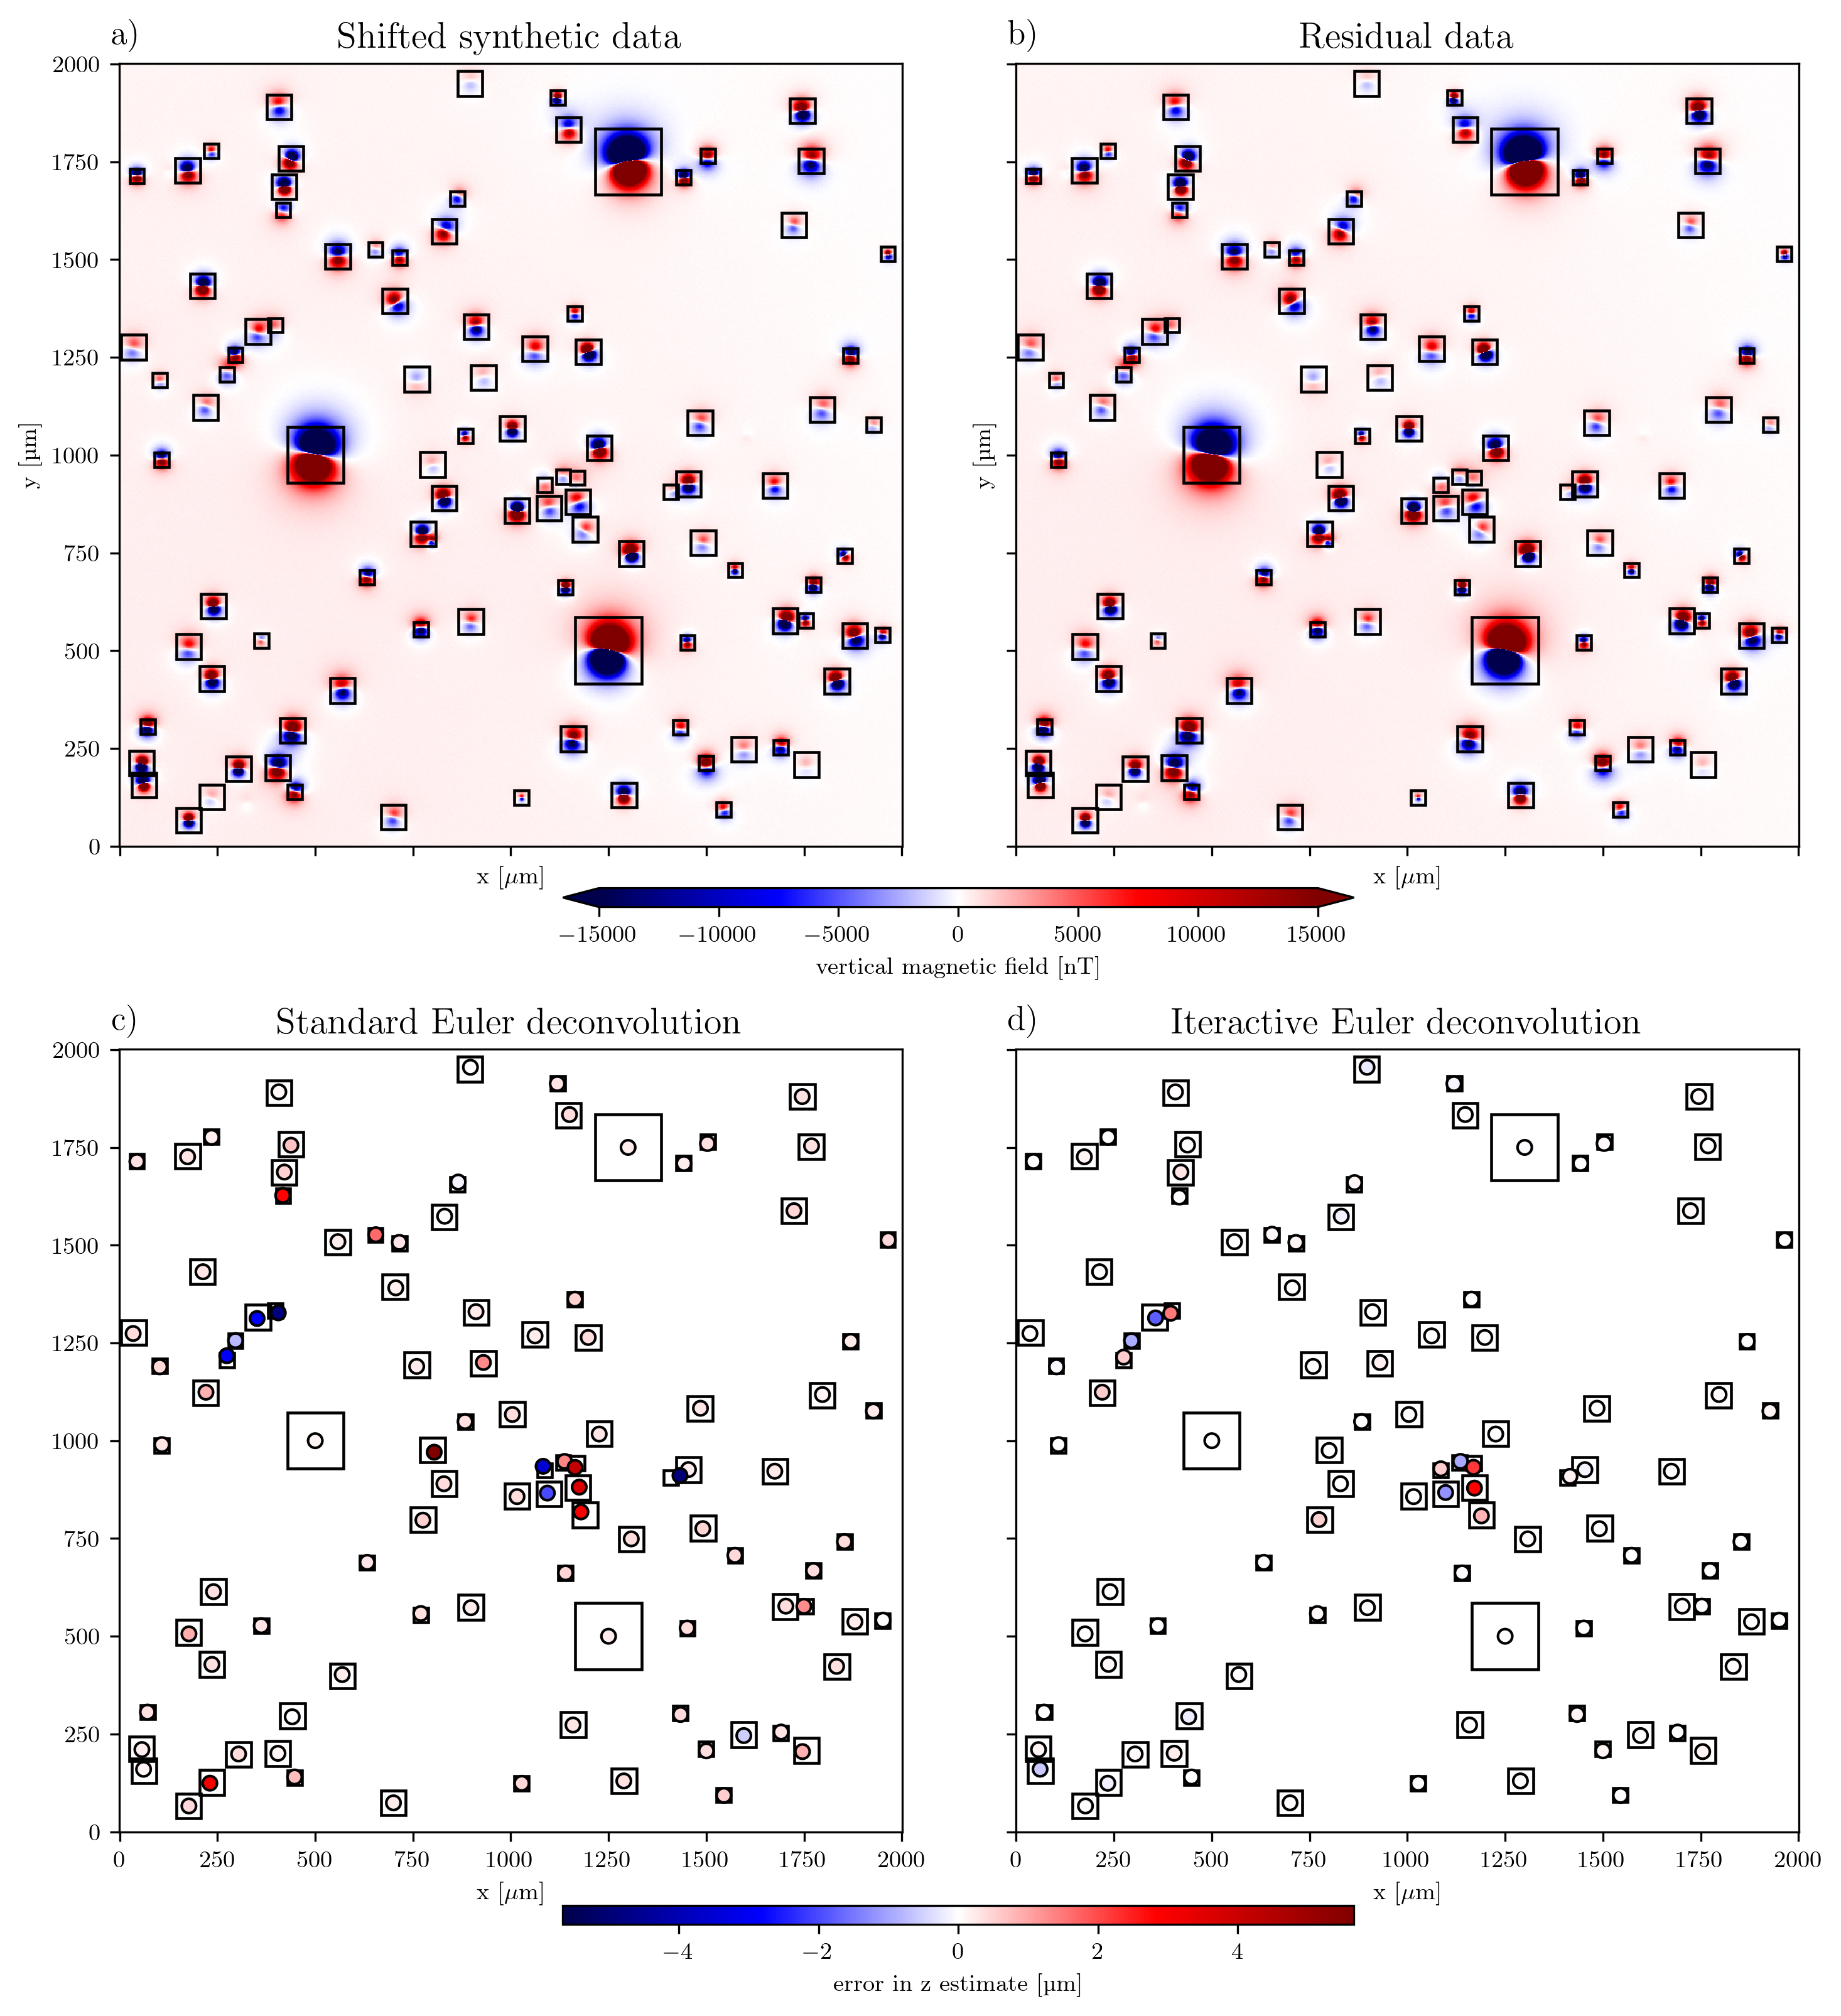
\includegraphics[width=1\linewidth]{figures/euler-comparion-2.png}
  \caption{
    % Addressing computational challenges in magnetic microscopy with extensive datasets.
    % a) Complete synthetic dataset featuring all N observation points including areas lacking relevant information.
    % b) Streamlining data through pre-selected windows reduces the dataset size for inversion, ensuring efficiency without compromising final results.
      }
  \label{euler2}
\end{figure}

Figure~\ref{inversion2} succinctly presents a comprehensive comparison encompassing angular misfit, magnetic moment misfit, and the r-squared score. The comparison is made across standard inversion results (Figures~\ref{inversion2}a-c), iterative inversion results for interfering sources (Figures~\ref{inversion2}d-f), interference with $b_z$ (Figures~\ref{inversion2}g-i), and interfering sources using the vertical derivative (Figures~\ref{inversion2}j-l). Differently from what was observed in the previous subsection, only the iterative and interfering sources using vertical derivative techniques consistently outperformed the standard method. Both techniques remained unaffected by the shift in the magnetic field, as well as the standard one. However, this pattern somehow changed for the interference source using $b_z$. Even though this technique yielded errors seemingly lower than the ones from the standard methodology, concerning the magnetic direction and moment misfit, it also demonstrated high variability in the results (not shown here) according to the shift in the magnetic field and the regional-residual separation technique used. For example, comparing the magnetic grains in the upper left region of Figure~\ref{euler2}b with Figure~\ref{inversion2}g it is clear that the sudden increase in the direction misfit is closely related to the region where the polynomial fit failed to remove the long-wavelength interference. This is also reflected in the r-squared score (Figure~\ref{inversion2}i), which makes this specific approach highly dependent on an ideal separation method. Based on this scenario, it seems that the iterative and interfering sources using the vertical derivative approaches might be more reliable for magnetic microscopy studies.

\begin{figure}[tb!]
  \centering
  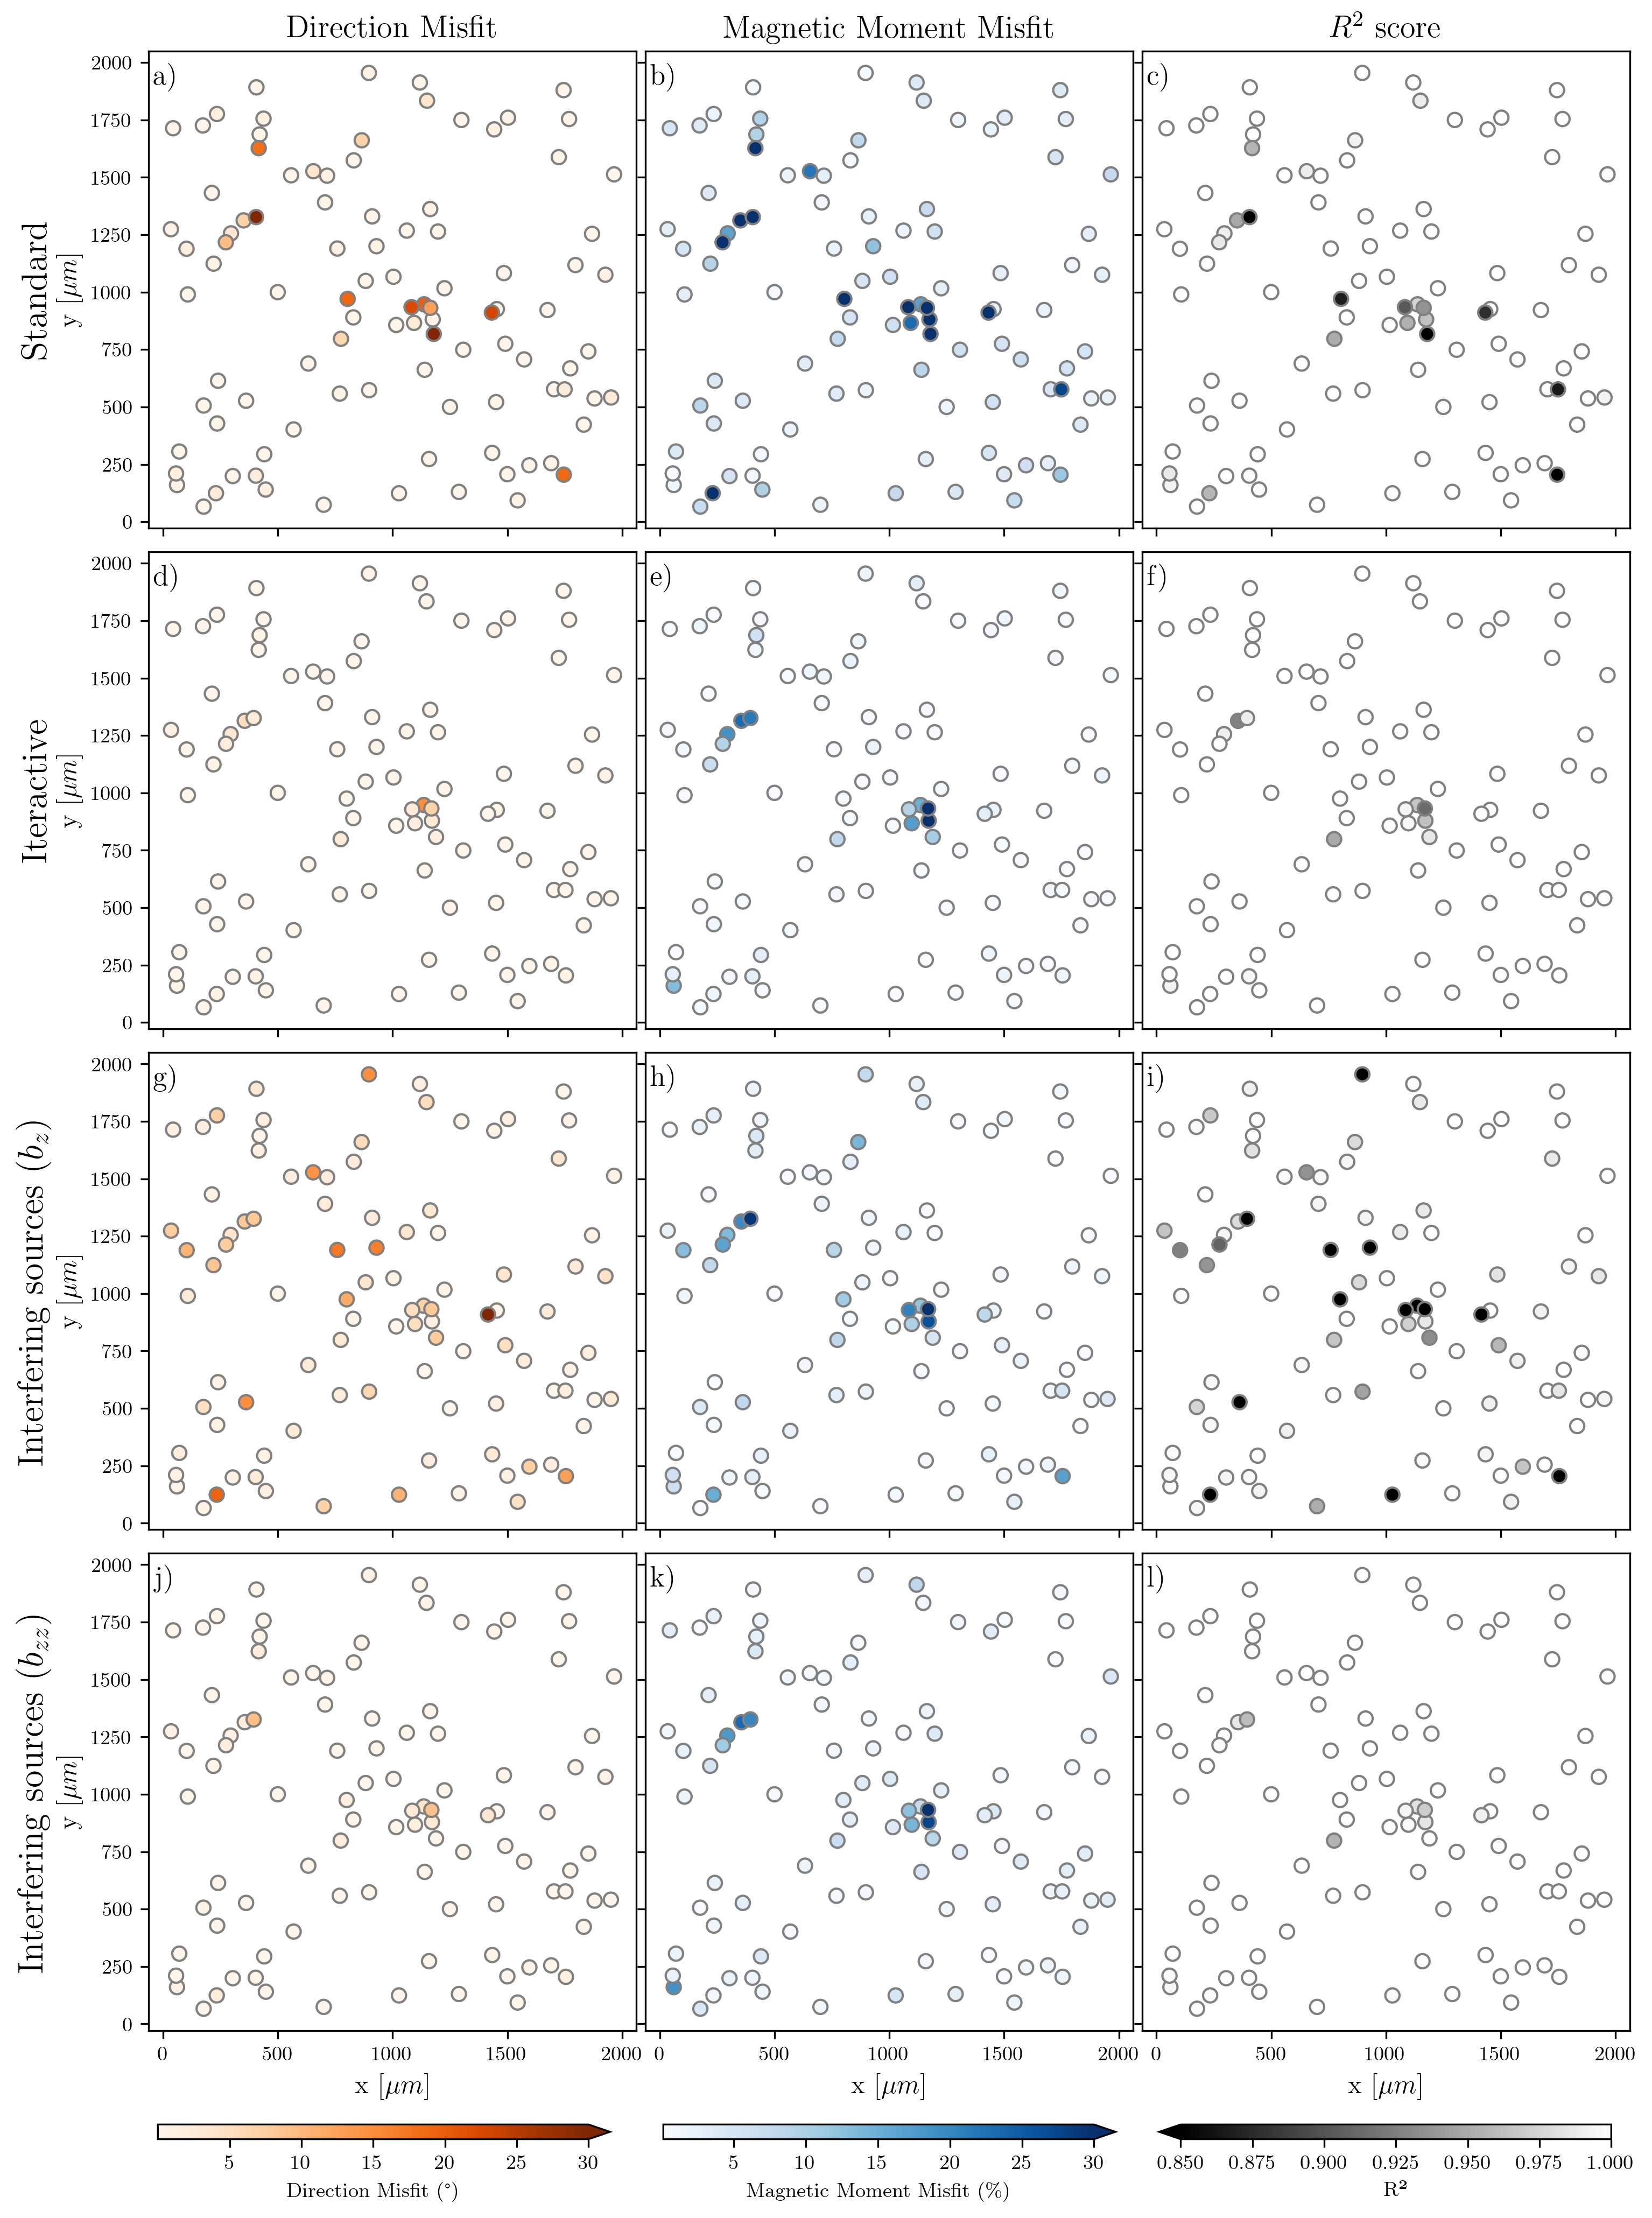
\includegraphics[width=1\linewidth]{figures/inversion-comparion-2.png}
  \caption{
    % Addressing computational challenges in magnetic microscopy with extensive datasets.
    % a) Complete synthetic dataset featuring all N observation points including areas lacking relevant information.
    % b) Streamlining data through pre-selected windows reduces the dataset size for inversion, ensuring efficiency without compromising final results.
      }
  \label{inversion2}
\end{figure}

% In all the synthetic and real data analyzed in this paper, the vertical derivatives were computed using the central finite difference equation (Equation x).
%%%%%%%%%%%%%%%%%%%%%%%%%%%%%%%%%%%%%%%%%%%%%%%%%%%%%%%%%%%%%%%%%%%%%%%%%%%%%%%
\section{Real data application}

\begin{figure}[tb!]
  \centering
  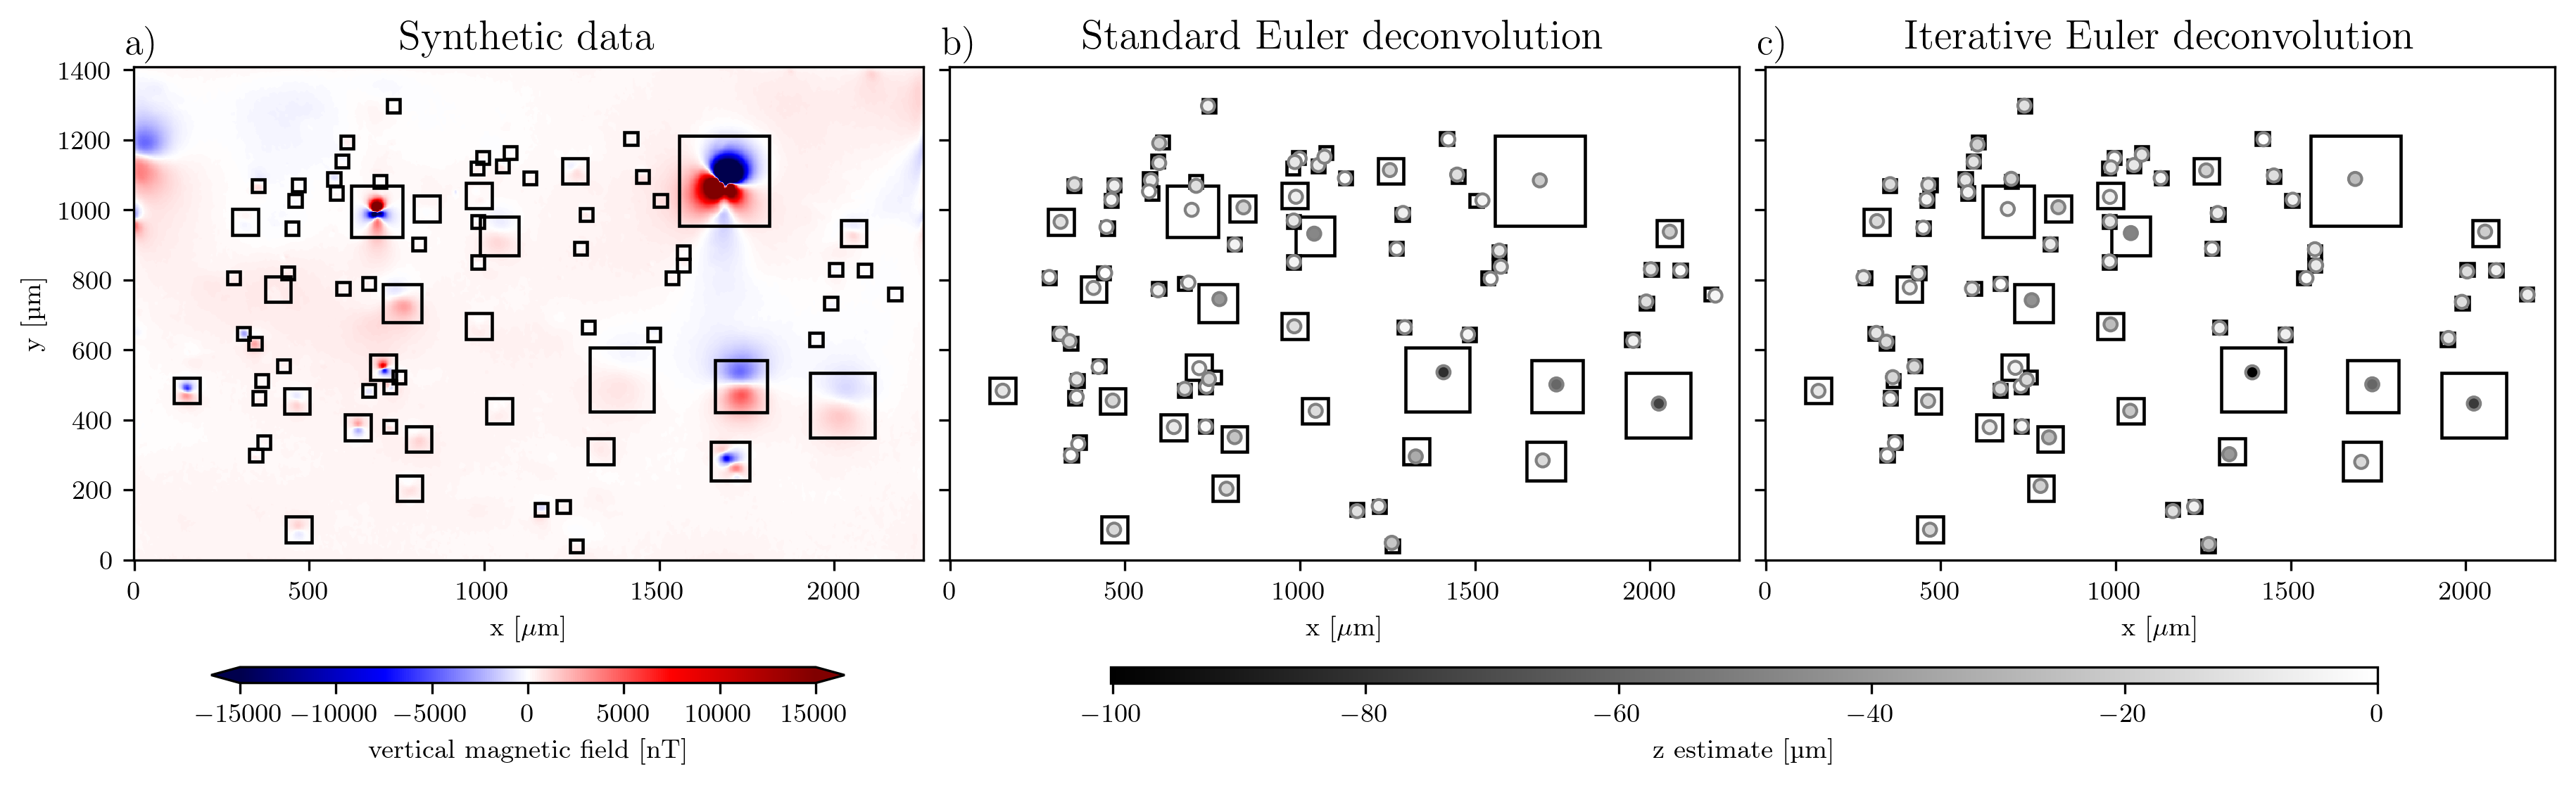
\includegraphics[width=1\linewidth]{paper/figures/euler-comparion-real.png}
  \caption{
    % Addressing computational challenges in magnetic microscopy with extensive datasets.
    % a) Complete synthetic dataset featuring all N observation points including areas lacking relevant information.
    % b) Streamlining data through pre-selected windows reduces the dataset size for inversion, ensuring efficiency without compromising final results.
      }
  \label{real-data-euler}
\end{figure}

\begin{figure}[tb!]
  \centering
  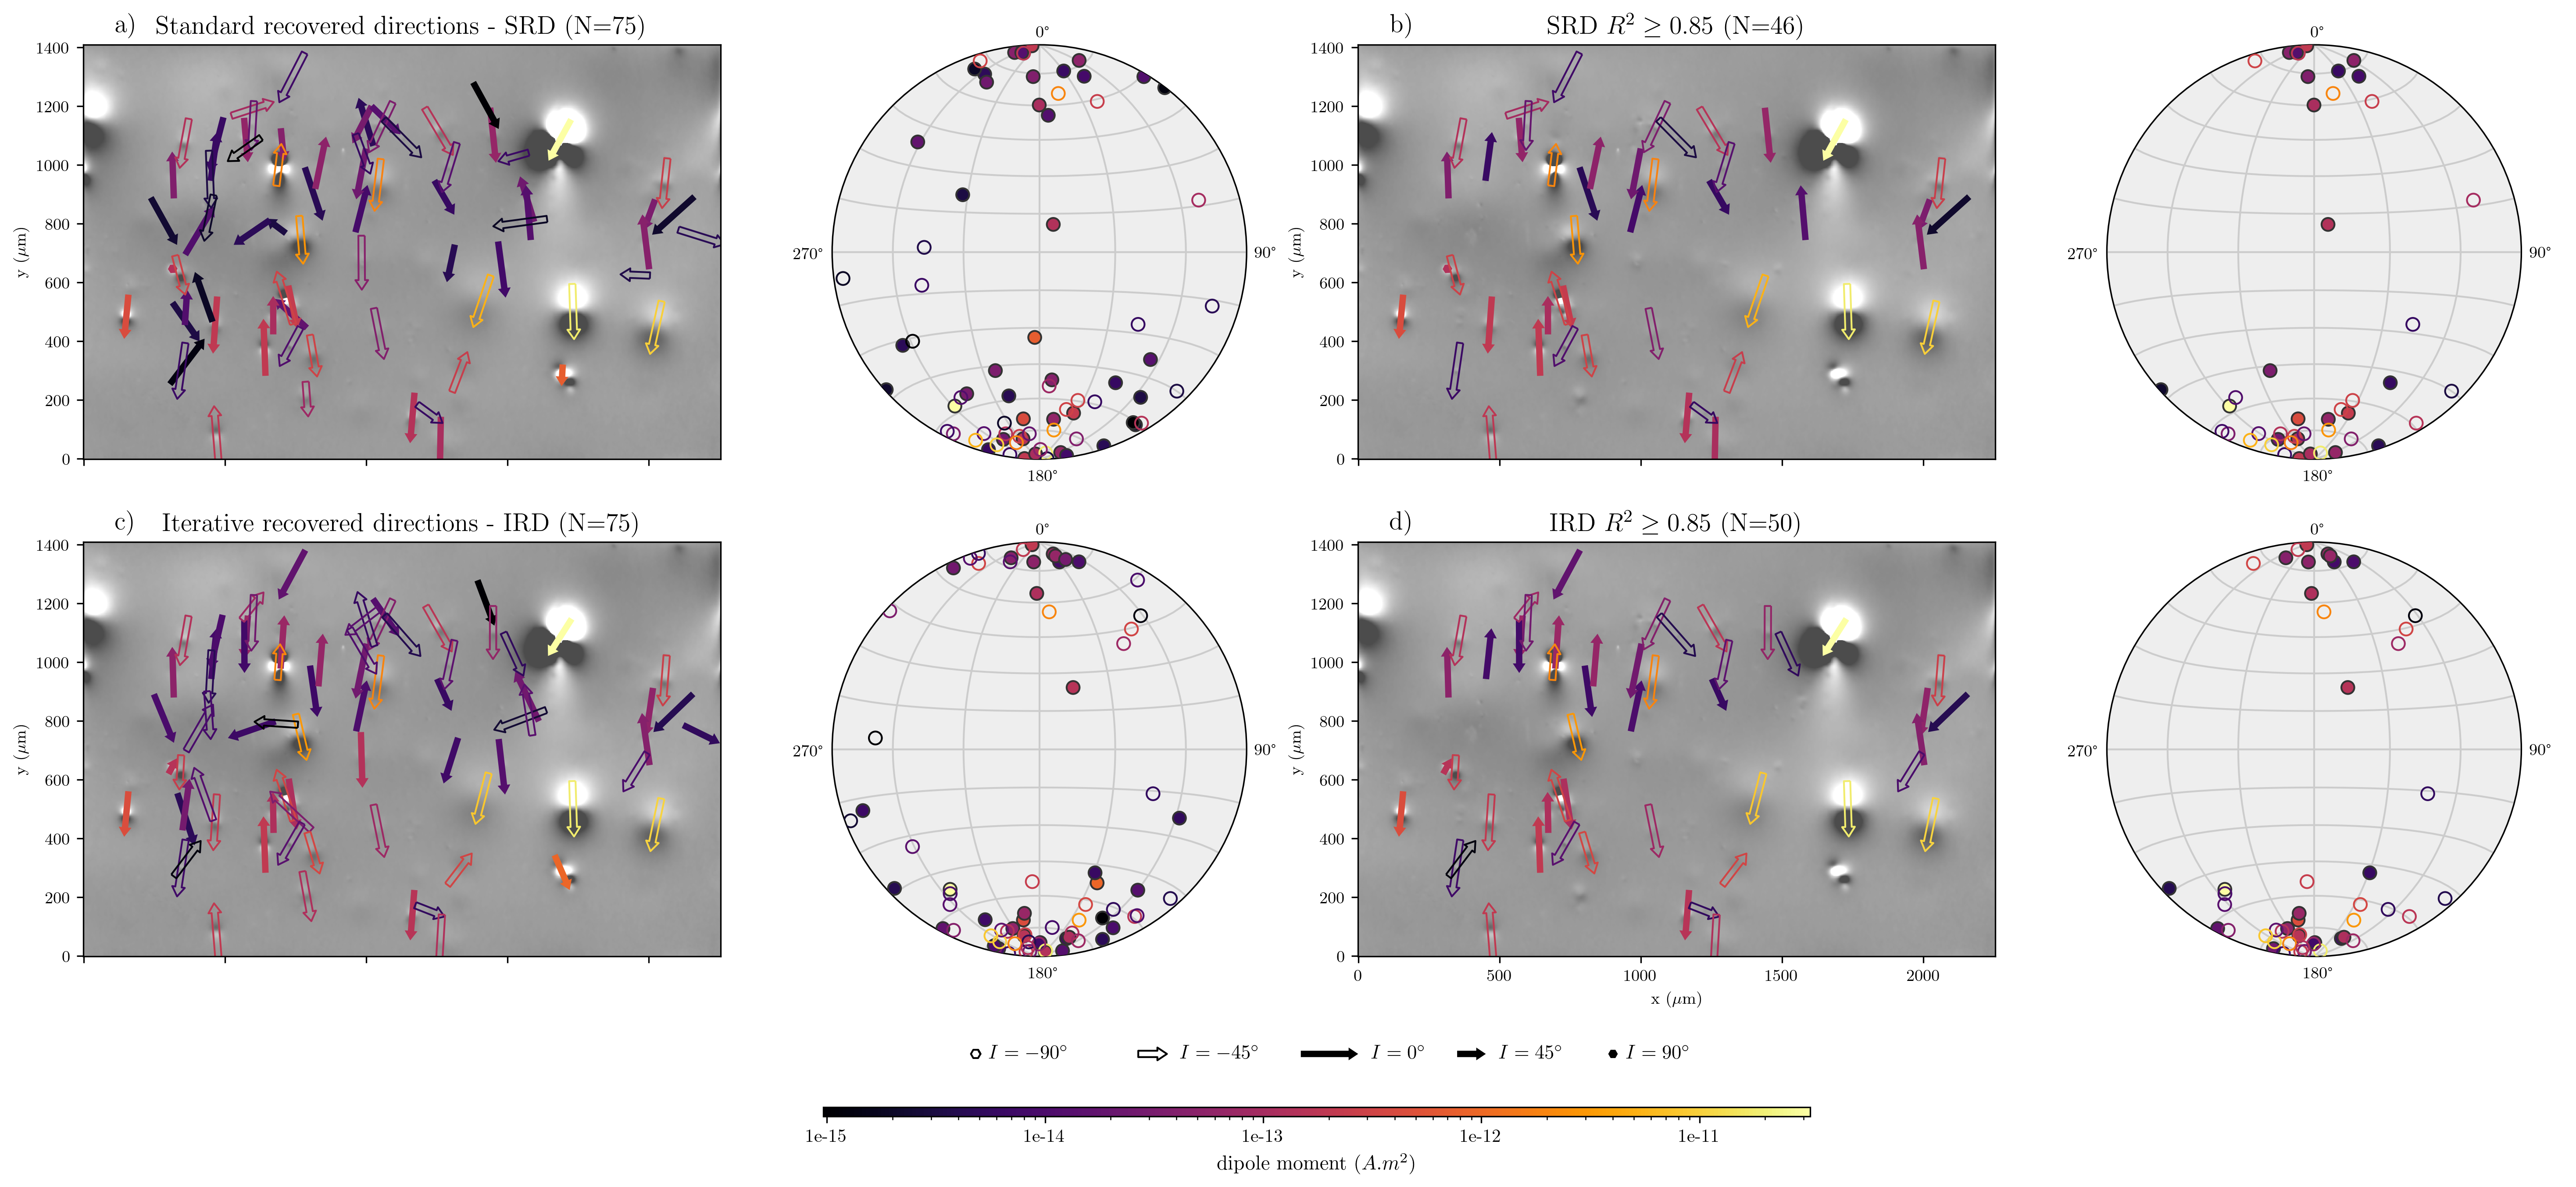
\includegraphics[width=1\linewidth]{paper/figures/real-data-stereograms.png}
  \caption{
    % Addressing computational challenges in magnetic microscopy with extensive datasets.
    % a) Complete synthetic dataset featuring all N observation points including areas lacking relevant information.
    % b) Streamlining data through pre-selected windows reduces the dataset size for inversion, ensuring efficiency without compromising final results.
      }
  \label{real-data-stereograms}
\end{figure}
%%%%%%%%%%%%%%%%%%%%%%%%%%%%%%%%%%%%%%%%%%%%%%%%%%%%%%%%%%%%%%%%%%%%%%%%%%%%%%%
\section{Discussions}


%%%%%%%%%%%%%%%%%%%%%%%%%%%%%%%%%%%%%%%%%%%%%%%%%%%%%%%%%%%%%%%%%%%%%%%%%%%%%%%
\section{Conclusion}



%%%%%%%%%%%%%%%%%%%%%%%%%%%%%%%%%%%%%%%%%%%%%%%%%%%%%%%%%%%%%%%%%%%%%%%%%%%%%%%
\section{Open research}

The Python source code used to produce all results and figures presented here, as well as supplemental figures and Jupyter notebooks, are available from \citet{sourcearchive}, which can also be found on \url{https://github.com/\GitHubRepository} under the MIT and CC-BY licenses.
The QDM magnetic microscopy data are available
from \citet{janinedata} under the CC-0 license.

The image re-scaling and blob detection through the Laplacian of Gaussian
methods were performed with the scikit-image library \citep{VanderWalt2014}.
We also used matplotlib \citep{Hunter2007} and mplstereonet \citep{mplstereonet}
for generating figures and stereograms.
Basic calculations were performed using Numpy \citep{Harris2020} and Scipy
\citep{2020SciPy-NMeth}.
Verde \citep{verde2018} was used to generate data grids.
Upward continuation was performed using Harmonica \citep{harmonica2020}.
The Choclo library \citep{choclo2022} provided kernel functions used in the
forward and inverse problems.
The Numba just-in-time compilation library \citep{lam2015numba} was used to
speed-up calculations.
Lastly, the xarray library \citep{hoyer2017xarray} offered a fast and powerful
tool for working with multi-dimensional datasets allowing an easy way of data
visualization and extraction with advanced indexing techniques.



%%%%%%%%%%%%%%%%%%%%%%%%%%%%%%%%%%%%%%%%%%%%%%%%%%%%%%%%%%%%%%%%%%%%%%%%%%%%%%%
\section{Acknowledgements}

We are indebted to the developers and maintainers of the open-source software
without which this work would not have been possible.
This research was supported by
grant 162704/2021-6 from the Conselho Nacional de Desenvolvimento Científico e Tecnológico (CNPq),
grant 2021/08379-5 from the Fundação de Amparo à Pesquisa do Estado de São Paulo (FAPESP),
grant PRPI 22.1.09345.01.2 from Universidade de São Paulo,
and grant IES\textbackslash{}R3\textbackslash{}213141 from the Royal Society.
The opinions, hypotheses, and conclusions or recommendations expressed in this
material are the responsibility of the authors and do not necessarily reflect
the views of FAPESP.
